% Preview source code

%% LyX 2.0.6 created this file.  For more info, see http://www.lyx.org/.
%% Do not edit unless you really know what you are doing.
\documentclass[english]{article}
\usepackage[latin9]{inputenc}
\usepackage[a4paper]{geometry}
\geometry{verbose,tmargin=1in,bmargin=1in,headheight=1in,headsep=1in}
\usepackage{float}
\usepackage{amsmath}
\usepackage{amssymb}
\usepackage{graphicx}

\makeatletter

%%%%%%%%%%%%%%%%%%%%%%%%%%%%%% LyX specific LaTeX commands.
%% Because html converters don't know tabularnewline
\providecommand{\tabularnewline}{\\}

%%%%%%%%%%%%%%%%%%%%%%%%%%%%%% User specified LaTeX commands.


\usepackage{amsthm}



%%%%%%%%%%%%%%%%%%%%%%%%%%%%%% LyX specific LaTeX commands.
%% Because html converters don't know tabularnewline
\providecommand{\tabularnewline}{\\}

%%%%%%%%%%%%%%%%%%%%%%%%%%%%%% Textclass specific LaTeX commands.
\numberwithin{equation}{section}
\numberwithin{figure}{section}



\usepackage{babel}

\makeatother

\usepackage{babel}
\begin{document}

\title{Future Virtual Particle Method for Pedestrian Navigation}


\author{Castiglione Gonzalo, Agustin Marseillan, Daniel Parisi}
\maketitle
\begin{abstract}
We present a novel method to simulate virtual pedestrians based on
the social force model. In our model, each pedestrian has a point
in front of him called Future Virtual Particle (FVP) which represents
where the pedestrian is headed to and at what speed. 
\end{abstract}
keywords:

pedestrian, collision avoidance, future virtual particle, force model

\pagebreak{}


\section{Introduction}


\subsection{Motivation and previous work}

Navigation of biological, sinthetic or virtual agents is a relevant
problem in several fields such as pedestrian dynamics, moving robots
and animation of characters for videogames and motion pictures.

Modelling and simulating the displacement of agents through arbitrarily
complex environments may be stated in an hierarchical structure of
mechanisms depending mainly on the distance from the agent. This level
has been named, from closer to further, as operational (walking, lowest
level physical-computational model for displacement), tactical (way-finding,
route choice) and strategic (general activity planning) {[}Hoogonen
and Bovy 2004{]}. These levels are not independent, factors affecting
one level may impact in the following and vice-versa, for example,
the route choice may vary due to congestion of agents produced from
previous route choice and walking behavior. Also, obstacles can impact
on the operational level or tactical level depending on the particular
geometry of the environment. The particular mechanism we want to address
is the avoidance of obstacles being fixed or moving (another agent)
which involves operational and tactical aspects of the navigation.

A general approach is to take an existing operational model and equip
it with a higher level model which allows better and smoother collision
avoidance behavior. Existing low level models can be taken from pedestrian
dynamics field and in general this models can be classified into rule
based and force based, discrete and continuous space description,
etc. {[}Schadschneider 2009{]}.

A famous example of continuous and force based model is the Social
Force Model {[}Helbing 1995, 2000{]}. In this model the dynamic for
virtual pedestrians is derived from the Newton equation's considering
the total force exerted over each agent is the result of three forces:
Contact, Social and Driving Force. While the driving force points
towards the final objective of each pedestrian, the social force is
repulsive and acts as a kind of collision avoidance force. However
this social force term introduces several artifices in some configurations
{[}see for example Lakoba et al. 2005, Parisi et al 2009{]}.

Cellular automaton models make use of a spatial grid, which can be
occupied or empty, along with a set of rules determining the evolution
and conflict resolution of virtual pedestrians moving over the cells
of the grid. An emblematic cellular automaton model is the one proposed
by Kirchner and Schadschneider {[}2002{]}.

Hybrid models have also been proposed such as the Contractile Particle
Model {[}Baglietto and Parisi, 2011{]} in which a continuous description
of the space is combined with a set of simple rules governing the
dynamics of the system.

The basic operational model -as the ones described above- can be improved
if higher level mechanisms were added to manage more complex issues
as efficient avoidance. Some recent examples can be found in the literature.

Karamouzas et al. (2009) proposed a method for collision avoidance
modifying the social force model, basically, replacing the social
force term by a new ``evasive\textquotedblright{} force which tends
to avoid future collisions. The magnitude and direction of this force
is calculated considering the predictions of these possible collisions.

Kretz et al. 2011 have arrised the point that the key ingredient in
social force model is the driving force instead of interaction force,
so in this work the authors propose a method for dynamically adjusting
the desired velocity following the gradient of a field given by a
time map, in other words, the desired velocity is chosen as the quickest
path to the objective taking into account the geometry and other agents
(collision, congestion, jams, etc.). Also mounted on the SFM, Moussaad
et al. {[}2011{]} presented a model using ``cognitive heuristics''
to determine the norm and direction of the desired velocity for each
agent dynamically during the evolution of the system.

In the same line, we also proposed that the navigation capacity of
virtual agents should be concentrated in the on-line decision of the
desired velocity. Both direction and magnitude calculation of the
desired velocity are the key differences with the SFM.

The method proposed could be mounted on different basic displacement
models like the SFM or the CPM, in the present work we have chosen
the first one.


\subsection{Social Force Model}

The Social Force is a model presented by Helbing \cite{key-0,key-1}
in several publications. This paper will focus on the latest version
of the model \cite{key-1}. In his model, each pedestrian $i$ occupies
a circular area of radius $r_{i}$ and is governed by thee forces.
\[
\vec{F_{i}}=\vec{F_{D_{i}}}+\vec{F_{S_{i}}}+\vec{F_{G_{i}}}
\]


This forces are a measure for the internal motivations of the individual
to perform certain actions.

The first term is known as the ``Driving Force''. It's calculated
as follows:

\begin{equation}
\vec{F_{D_{i}}}=m_{i}\frac{v_{di}\vec{e_{i}}-\vec{v_{i}}}{\tau}\label{eq:driving-force}
\end{equation}


\begin{equation}
\vec{e_{i}}=\frac{\vec{x}_{i}^{k}-\vec{x}_{i}(t)}{||\vec{x}_{i}^{k}-\vec{x}_{i}(t)||}\label{eq:desired-direction}
\end{equation}


$\vec{F}_{D_{i}}$ represents the force that a pedestrian $i$ keeps
towards his desired velocity of motion.

$v_{di}$ is the desired speed for the pedestrian $i$.

$\vec{e}{}_{i}$ is the desired direction of motion of the pedestrian
$i$.

$\vec{v}{}_{i}$ is the current velocity of the pedestrian $i$.

$\vec{x}_{i}(t)$ is the actual position of the pedestrian $i$ at
the time $t$.

$x_{i}^{k}$ is the closest point from the goal (represented as an
area) to pedestrian $i$. \\


Figure \ref{fig:driving-force} shows an example of a pedestrian currently
moving in direction of $\vec{v}$ but adjusting its trajectory towards
\textbf{$X$}.

\begin{figure}[H]
\begin{centering}
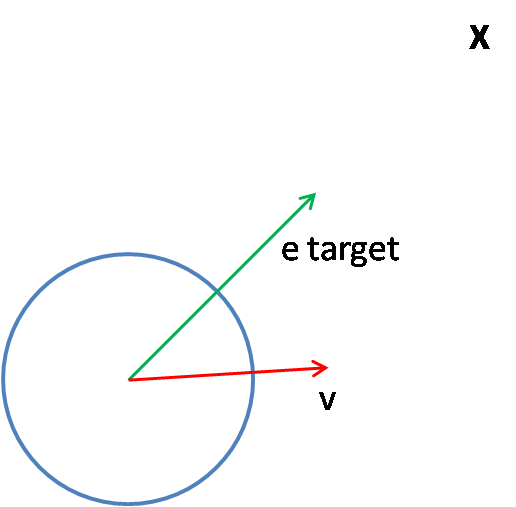
\includegraphics[scale=0.4]{pics/sfm/drivingforce} 
\par\end{centering}

\caption{\label{fig:driving-force}Driving force}
\end{figure}


\vspace{1cm}


The second term is known as the ``Social force''. It's calculated
as follows:

\begin{equation}
\vec{F}_{S_{i}}=\sum_{j=1,j\ne i}^{N_{P}}Aexp(-\frac{\epsilon_{ij}}{B})\,\vec{e}_{ij}^{n}\label{eq:social-force}
\end{equation}


$\vec{F}_{S_{i}}$ represents the fact that a pedestrian keeps a certain
distance to other pedestrians and borders.

$N_{p}$ is the number of existing pedestrians.

$A$ and $B$ are constants determined by simulations.

$\epsilon_{ij}$ is the distance from $x_{i}$ towards $x_{j}$.

$\vec{e}_{ij}^{n}$ is the unit vector from $x_{i}$ towards $x_{j}$.\\


Figure \ref{fig:Social-Force} shows \ref{eq:social-force} graphically.

\begin{figure}[H]
\begin{centering}
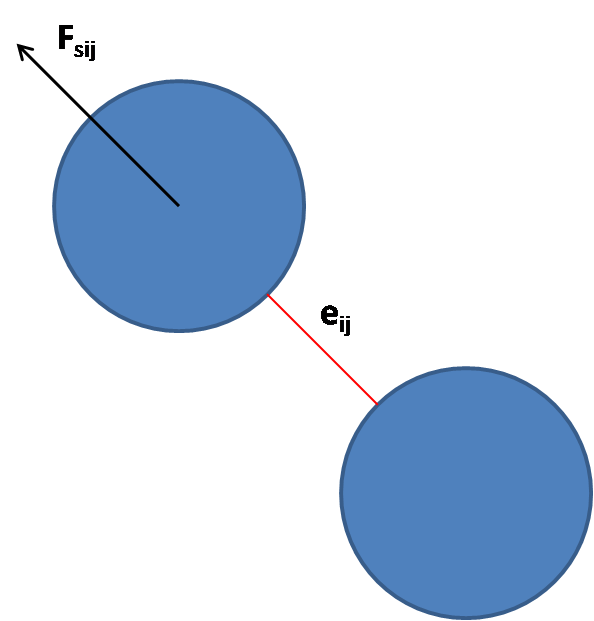
\includegraphics[scale=0.4]{pics/sfm/sf} 
\par\end{centering}

\caption{Social Force\label{fig:Social-Force}}
\end{figure}


\vspace{1cm}


The third term is known as the ``Granular force''. It's calculated
as follows:

\begin{equation}
\vec{F}_{G_{i}}=\sum_{j=1,j\ne i}^{N_{P}}[-\epsilon_{ij}k_{n}\vec{e}_{ij}^{n}+v_{ij}^{t}\epsilon_{ij}k_{t}\vec{e}_{ij}^{t}]\, g(\epsilon_{ij})\label{eq:granular-force}
\end{equation}


$\vec{F}_{G_{i}}$ represents the physical force that a pedestrian
suffers when colliding with another object (pedestrian or wall).

$k_{n}$ and $k_{t}$ are the normal and tangential friction coeficient
respectively.

$g$ is ???\\


Figure \ref{fig:colliding-pedestrians} shows \ref{eq:granular-force}
graphically.

\begin{figure}[H]
\begin{centering}
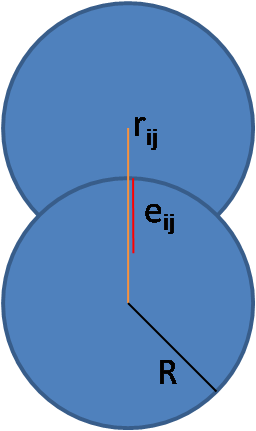
\includegraphics[scale=0.4]{pics/sfm/ganular} 
\par\end{centering}

\caption{Colliding pedestrians\label{fig:colliding-pedestrians}}
\end{figure}


\vspace{1cm}


Afterwards $\vec{F}_{i}$ is calculated on each simulation step for
each of the pedestrians and applied until all of them had reached
their goal.

Fixed parameter values:

\begin{center}
\begin{tabular}{|c|c|}
\hline 
Name & Value\tabularnewline
\hline 
\hline 
$A$ & $2000\,[N]$\tabularnewline
\hline 
$B$ & $0.08\,[m]$\tabularnewline
\hline 
$k_{n}$ & $1.2\,10^{5}\,[\frac{N}{m}]$\tabularnewline
\hline 
$k_{t}$ & $2.4\,10^{5}\,[\frac{kg}{m/s}]$\tabularnewline
\hline 
$\tau$ & $0.5\,[s]$\tabularnewline
\hline 
\end{tabular}
\par\end{center}


\subsection{Future Virtual Particle Model}

Given that the SFM adds a fictional force on pedestrians, navigation
doesn't resemble reality for high pedestrian densities. Also, SFM
didn't have the same values as well known metrics for real-case scenarios
such as the flow of pedestrians going out a door and the fundamental
diagram.

Because of this, we present a new model in which the social force
from equation \ref{eq:driving-force} affecting directly on each pedestrian
is eliminated and replaced with a desire force facing a short term
objective. This force is created using equation \ref{eq:desired-direction}
replacing $r_{i}^{k}$ with the vector facing the closest point on
the short term objective area.


\section{The Model}


\subsection{Hipotesis}

The main effects that govern the motion of a pedestrian are the same
as Helbin's \cite{key-0,key-1}: 
\begin{enumerate}
\item The pedestrian wants to reach his goal in the shortest possible path. 
\item The pedestrian's movement is influenced by other pedestrians. Depending
on the distance between the two of them and the predicted trajectory,
the pedestrian feels the need to change his route to be able to avoid
the other pedestrians. It is because of this effect that pedestrians
will need to recalculate their route as new pedestrians get closer
to them. 
\item Movement speed will be influenced by the presence of other pedestrians
and obstacles.
\end{enumerate}

\subsection{Geometrical definition}

A pedestrian is defined as follows: 
\begin{itemize}
\item Circular shape


Represents the personal space of a pedetrian. The value of the radio
is generated randomly for each pedestrian. The range of values is
distributed uniformly in $[0.25,0.29]$$[cm]$.

\item Long term objective


Represented by a static area. When it is touched by a pedestrian,
it is considered as accomplished. Multiple objectives may by defined
in a list, in this case, each of them must be reached in order.

\item Short term objective


Called future virtual particle (FVP), it represents a point at a relative
distance from the pedestrian's center. It's a dynamic objective.


It is defined as a $1\,[kg]$ mass. Not collisionable.

\item Desired speed


This is the speed the pedestrian would walk if he/she was alone. This
represents the constant $v_{di}$ in ecuation \ref{eq:driving-force}.
It takes a different value for each pedestrian. Varies with a uniform
distribution between $[1.2,1.4]\,[m/s]$.

\item Reaction distance ($RD$)


Maximum distance between a pedestrian and his FVP, it represents the
distance at which a real pedestrian would react from an obstacle.

\end{itemize}
\vspace{1cm}


\begin{figure}[H]
\centering{}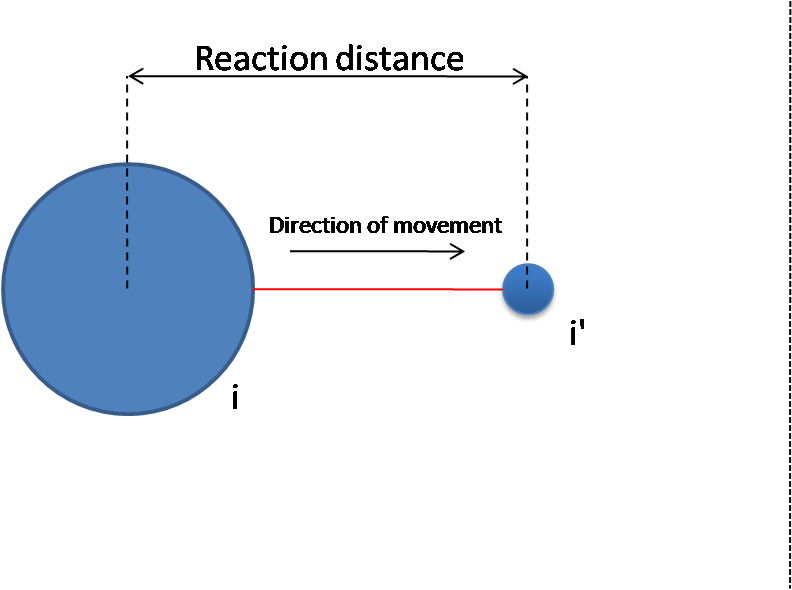
\includegraphics[scale=0.5]{pics/pedestrian-top}\caption{\label{fig:pedestrian-geometry}Pedestrian geometry}
\end{figure}


For the sake of clarity. A single pedestrian will be named after a
letter (i.e: $i$ or $j$) and the same letter with a apostrophe will
represent it's FVP (i.e: $i'$ or $j'$)\\


Figure \ref{fig:pedestrian-vectors} shows all the vectorial definition
that will be used:

\begin{figure}[H]
\centering{}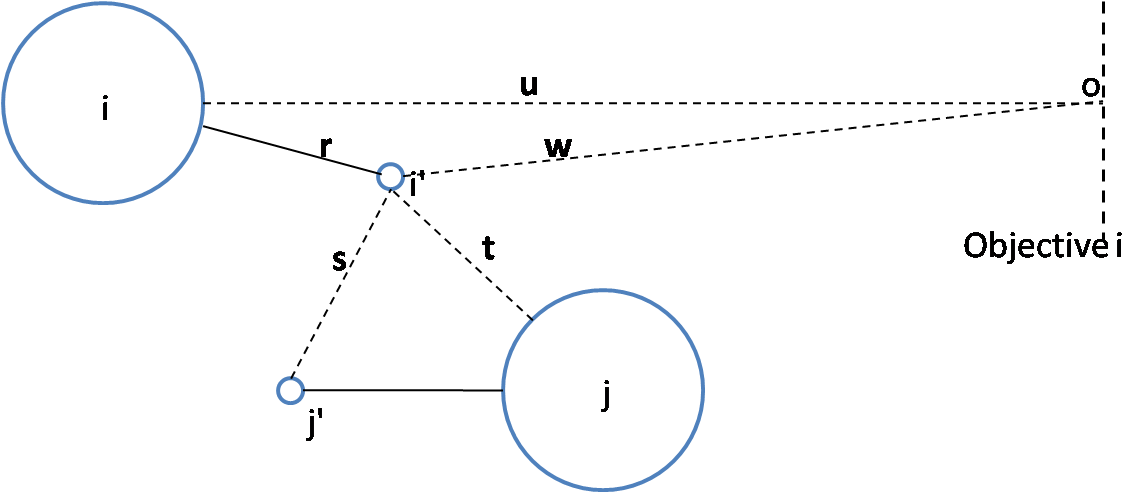
\includegraphics[scale=0.5]{pics/geometry}\caption{\label{fig:pedestrian-vectors}Vectorial definitions}
\end{figure}


\vspace{1cm}



\subsection{Dynamics of the FVP Model}

In this section all the forces acting on the FVPM will be defined


\subsubsection{Calculatin of forces}
\begin{itemize}
\item Dynamic of the FVP


Each pedestrian has to reach the long term objective at some point,
to ensure this, the FVP needs to be aligned with the shortest path
to the long term objective $\mathbf{o}$. On the other hand, there
are sometimes obstacles in the way, which will make this impossible,
in this cases, the route will have to change depending on the situation.


To model this situations, two types of forces act over the FVP:
\begin{itemize}
\item Internal force \\
 \\
 This force will guide the pedestrian on the shortest path $\mathbf{ox_{i}}$.
This force is modeled using two springs: 


The first spring starts on $x_{i}$, ends on $x_{i}'$ and has a steady
distance of $RD$ with a spring constant $K_{s}(\theta)$ where $\theta$
is the angle between $\mathbf{u}$ and $\mathbf{r}$. With this spring
the FVP will tend to always be at $RD$ distance from the pedestrian.
Because a pedestrian always tries to reach his goal in the shortest
possible path (hypothesis 1), if it has to take a big detour of his
ideal path, it will try to reduce his velocity drastically in order
to avoid making a long travel. To recreate this, the spring constant
has to be dependant of the deviation angle. 
\[
K_{s}(\theta)=\frac{K_{2}}{\theta}
\]



The second spring starts on $x_{i'}$ and ends on the point at distance
$RD$ on vector $\mathbf{x_{i}o}$ with a spring constant $K_{1}$.
This spring represents how much the pedestrian wants to reach his
target. A larger spring constant will force a more straight path,
but possible with more collisions on its way. In order to avoid an
oscillatory movement (i.e: with a single pedestrian), a damping $\gamma$
was added to this spring.\\



Given pedestrian $i$, the equation for his internal force is:


\begin{equation}
F_{internal}(i)=K_{1}*(|r|-RD)+K_{2}(\theta_{i})+K_{2}(\theta_{i})*(???)
\end{equation}



$\iffalse F_{s}(r,\theta)=K_{s}(\theta)\frac{\vec{ii'}}{\mid\vec{ii'}\mid}(r_{max}-r_{ii'})\fi$


\begin{figure}[H]
\centering{}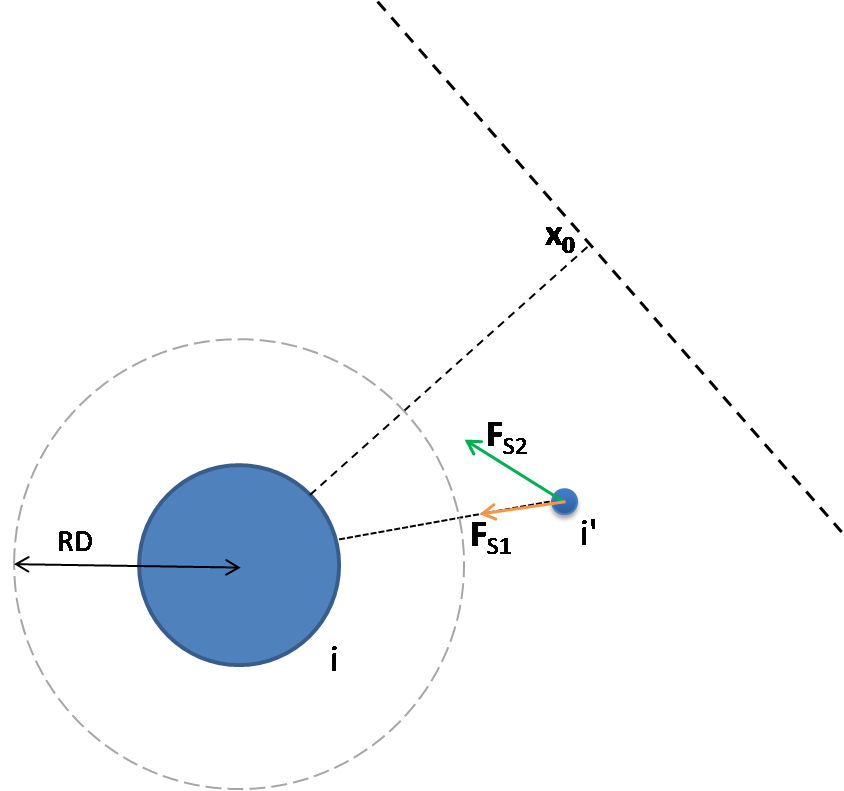
\includegraphics[scale=0.5]{pics/pedestrian-internal-forces}\caption{Pedestrian internal forces}
\end{figure}


\item Avoidance forces \\
 \\
 This force will produce avoidance movements when obstactes are detected
on the path. The magnitude of this force is calculated using two factors:
\\
 The first factor is calculated for each of the pedestrian $j$ ($j\neq i$)
who is in the range of sight of pedestrian $i$. This restriction
is verified using the following condition:


\[
\mathbf{r_{ii'}}\bullet\mathbf{r_{ij'}}<0
\]



This filter represents the fact that a pedestrian (in most cases)
does not make decisions based on obstacles behind him. Hence, they
are ignored. The formula for the external forces that the FVP $i$
feels is defined as follows


\[
F_{ext}(i)=\sum_{j}F_{i',j'}+F_{i'j}=\sum_{j}(\alpha_{ff}e^{-dist(i',j')/\beta_{ff}})+\sum_{j}(\alpha_{fp}e^{-dist(i',j')/\beta_{fp}})
\]



where $\alpha_{x}$ and $\beta_{x}$ are predefined constants.


The first term of the sum acts as a repulsion force between $i$ and
$j$ FVPs, resulting in the avoidance of a future collision. The second
term uses this same principle but calculates the repulsion force between
$j's$ FVP and $i$. Repulsion against walls is calculated in the
same way, by using the closest point between the FVP and the wall
and special values for $\alpha_{fw}$ and $\beta_{fw}$ for the calculation.


\iffalse The first term of the sum represents the fact that $i$
does not want to be in the same location as $j$ in the near future.
Note that $j'$ represents the predicted location of $j$ inferred
by another pedestrian (in this case, $i$) and because of this, it
moves it's near future away of that predicted location. The second
term, represents the same fact but taking in mind the current location
of the pedestrian $j$. The same law applies to each of the walls
on the simulation, the difference is that the closest point on the
wall and and the future has to be calculated before applying the formula.
Also, the constants $\alpha_{fw}$ and $\beta_{fw}$ have different
values. \fi


Figure \ref{fig:External-forces-affecting} shows the external forces
that a pedestrian $i$ suffers because of another pedestrian ($j$)
and also the direction in which $i$ desires to move.


\begin{figure}[H]
\centering{}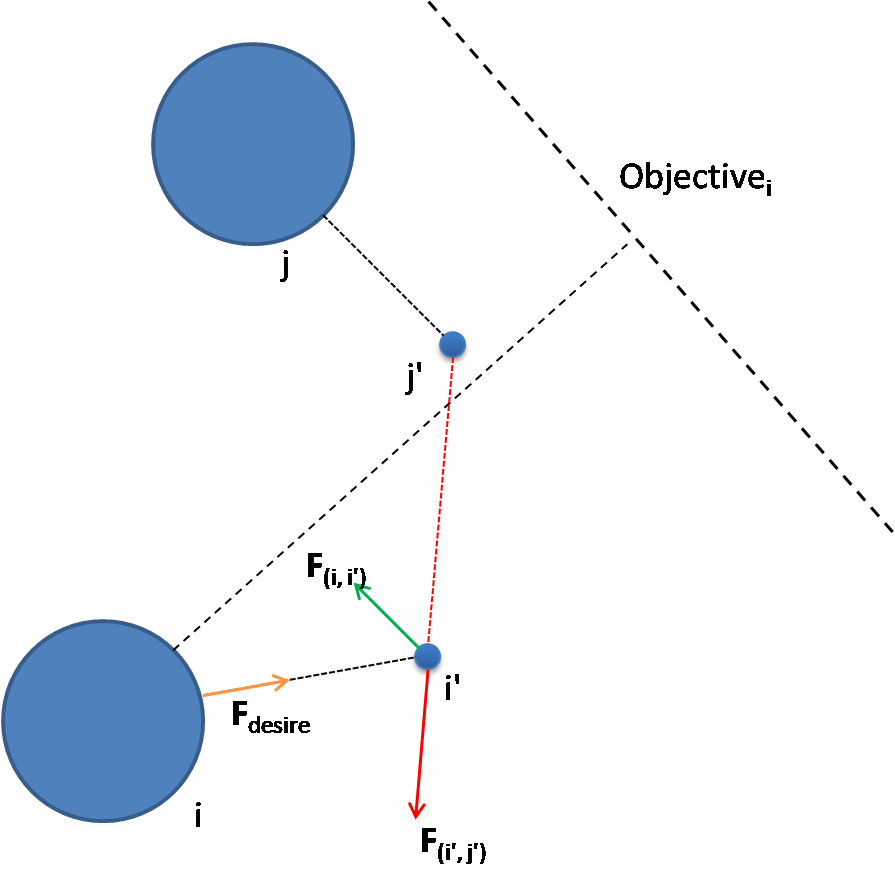
\includegraphics[scale=0.5]{pics/pedestrian-top-forces}\caption{\label{fig:External-forces-affecting}External forces affecting future
$i'$}
\end{figure}


\end{itemize}

After this, the final $F_{i'}$ is computed by adding all the terms.
$F_{i'}=F_{ext}(i)+F_{i\, s1}+F_{i\, s2}$.\\



To avoid high symetry situations, a low noise $P=10\%$ is added to
$F$. There are two ways to apply this noise: 
\begin{itemize}
\item Radial noise:

\begin{itemize}
\item A value $p$ is taken randomly from a uniform distribution $[-P,\, P]$
and calculate: $FL_{i'}=F_{i'}*p$ 
\item Angular noise:

\begin{itemize}
\item A value $sgn=\{-1,\,1\}$ is taken randomly from a uniform distribution
and a value $p$ from $[-P,\, P]$. Then $FA_{i'}=rotation(F_{i'},\,\pi*sgn)*p$
is calculated. 
\end{itemize}
\end{itemize}

At last, we find $F'_{i'}=F_{i'}+FL_{i'}+FA_{i'}$ and apply movement
equations.

\end{itemize}
\item Dynamic of the pedestrian


The pedestrian always wants to move in the direction his FVP is pointing
and its magnitude is defined as $F_{d}$ or driving force:


\[
\vec{F}_{desire_{i}}=m_{i}\frac{\frac{|\vec{ii'}|}{|\vec{r}_{max}|}\vec{e_{i}}-\vec{v}_{i}}{\tau}
\]



Where $\tau=0.5$


\textit{{*}It is important to note that the only deviation from the
SFM in this equation is the $k\vec{e}_{i}$ term. As described above,
this model focuses on improving the SFM through dynamically adjusting
the desired velocity.}

\end{itemize}

\subsubsection{Algorithm}

The pedestrian movement is calculated in four steps: 
\begin{enumerate}
\item Calculate forces for each FVP. 
\item Update positions for each FVP. 
\item Calculate forces for each pedestrian. 
\item Update positions for each pedestrian. 
\end{enumerate}

\section{Calibration}


\subsection{Metrics}

The results where compared to the SFM \cite{key-1}. The test scenarios
where crossing and hallway for they present the main types of symmetry
(90 degrees and 180 degrees respectively).

The metrics used where: 
\begin{enumerate}
\item Number of collisions


The total amount of collisions between pedestrians.

\item Total duration of collisions:


The sum of the duration of each collision.

\item Average walking speed:


The average of the average speed of each pedestrian.

\item Average travel time:


The average time that a pedestrian needed unit it reached the goal.

\item Average travel distance:


The average distance that a pedestrian traveled unit it reached the
goal.

\item Average turn angle:


The average angle turned by a pedestrian unit it reached the goal.

\end{enumerate}

\subsection{Values}

To calibrate the model, runs varying parameters were made. A wide
spectrum of values was covered, testing every combination of every
possible one. After seeing clear preferences towards certain values,
the values were refined within that scope. After numerous iterations
of this process, the values that best suit these metrics are$\alpha=800$
y $\beta=[0.65,\,085]$ uniformly distributed.

//TODO todos los demas parametros


\section{Results}

\vspace{1cm}


\begin{table}[H]
\centering{}%
\begin{tabular}{|c|c|c|c|c|c|c|}
\hline 
{\scriptsize{Values}}  & {\scriptsize{1}}  & {\scriptsize{2}}  & {\scriptsize{3}}  & {\scriptsize{4}}  & {\scriptsize{5}}  & {\scriptsize{6}}\tabularnewline
\hline 
\hline 
{\scriptsize{$\alpha=1000,\,\beta=[0.4,\,0.5]$}}  & {\scriptsize{(1.800, 0.748) }}  & {\scriptsize{(34.600, 8.333) }}  & {\scriptsize{(1.024, 0.016) }}  & {\scriptsize{(1.910, 0.022) }}  & {\scriptsize{(2.392, 0.005) }}  & {\scriptsize{(111.062, 19.122)}}\tabularnewline
\hline 
{\scriptsize{$\alpha=2000,\,\beta=0.08$}}  & {\scriptsize{(5.333, 2.625)}}  & {\scriptsize{(12.333, 8.340) }}  & {\scriptsize{(1.052, 0.003) }}  & {\scriptsize{(1.876, 0.003) }}  & {\scriptsize{(2.391, 0.002) }}  & {\scriptsize{(106.185, 13.778)}}\tabularnewline
\hline 
\end{tabular}\caption{Metrics comparing SFM vs FVPM. Average of $10$ runs.}
\end{table}


\textbf{// Poner Graficos indicando distancias y esquemas del future
y la particula. }


\section{Conclusions}

\textbf{// agregar al final futuras opciones que se abren con este
trabajo}

\pagebreak{}
\begin{thebibliography}{1}
\bibitem{key-0}Helbing, Dirk; Molnár, Péter (1995). ``Social force
model for pedestrian dynamics''.

\bibitem{key-1}Helbing, Dirk; Farkas, Illés; Vicsek, Tamás (2000).
``Simulating dynamical features of escape panic''

\bibitem{key-2}I. Karamouzas (2009). ``A Predictive Collision Avoidance
Model for Pedestrian Simulation''\end{thebibliography}

\end{document}

